% This is a default-selection of plugins that are used widely in this repo.

\documentclass[a4paper,10pt,fleqn]{article}
\usepackage[utf8]{inputenc}

% deutsche Trennmuster etc.
\usepackage[ngerman]{babel}
\usepackage[T1]{fontenc}

% mathematical simbols and fonts
\usepackage{mathtools} 
\usepackage{amssymb}
\usepackage{amsmath}
\usepackage{ntheorem}
\usepackage{polynom}
\usepackage{marvosym}
\usepackage{tabu}
\renewcommand*{\bmod}{\mathbin{\%}}
\everymath{\displaystyle}

\usepackage{multicol}
\usepackage{color}
\usepackage[usenames,dvipsnames]{xcolor}
\setlength{\columnsep}{1cm}
\setlength{\columnseprule}{0.25pt}
\def\columnseprulecolor{\color{gray}}
\usepackage{hyperref}

\usepackage[margin=1.5cm]{geometry}
\usepackage{graphicx}
\usepackage{pgfplots}
\pgfplotsset{compat=1.10}

%Code higlighting

\usepackage{minted}

% make lists more compact:
\newlength{\wideitemsep}
\setlength{\wideitemsep}{.5\itemsep}
\addtolength{\wideitemsep}{-5pt}
\let\olditem\item
\renewcommand{\item}{\setlength{\itemsep}{\wideitemsep}\olditem}
\renewcommand{\arraystretch}{1.25}

\title{Zusammenfassung AutoSpr}
\author{Fabian Hauser}
 
\begin{document}
\maketitle

\section{Varia}
Unterrichtszeiten: 12:00-12:30, 13:45-14:15, 14:20-14:50

Prüfung: Zusammenfassung $1m^2  = 8 \cdot A4$, Taschenrechner


\section{Notation}
Prädikat:	Aussagen

\subsection{Logik}
Siehe Seite 5 Script!

\subsection{Mengenlehre}

\section{Sprachen}

\subsection{Alphabet}
Definition : Nicht leere Menge von "Zeichen".

Zum Beispiel: $\Sigma = \{0, 1\}$, $\Sigma = \{1\}$, $\Delta = \{a,b,c,...,z\}$


\subsection{Wort}

Definition: Zeichenkette von Zeichen aus $\Sigma$: $w \in \Sigma^n = \Sigma \times \Sigma \times ... \times \Sigma$. Länge: $|w| = n$
\[
	\Sigma^0 = \{\varepsilon\}; \varepsilon = \text{ leeres Wort}
\]
\[
	\Sigma^\ast = \Sigma^0 \cup \Sigma^1 \cup ... \cup \Sigma^n = \bigcup^{\infty}_{k=0}{\sum^k}
\]

Im Zusammenhang mit der Sprache sind Zeichenketten bedeutungslos!


\paragraph{Beispiele}

\begin{align*}
\Sigma &= \{1\} & \Sigma^\ast &= \{\varepsilon, 1,11,111,1111,...\} \\
L &\subset \Sigma^\ast  & L &=\{1,11,1111,11111111,....\} = \{w \in \Sigma^\ast| |w|=2^k, k \in \mathbb{N}\}
\end{align*}

\subsection{Wortkombinationen}

Verkettung: $L_1$, $L_2$ Sprachen

\[
	L_1 L_2 = \{w_1 w_2 | w_1 \in L_1 \land w_2 \in L_2 \}
\]

$LL = L^2$, $L^n = L^{n-1}L, L^0 = \{\varepsilon\}$


Für Wortkombinationen wird ein NEA benötigt, welcher die Automaten der einzelnen Sprachen mit $\varepsilon$-Übergängen verknüpft.

\[
	L^\ast = L^0 \cup L^1 \cup ... = \bigcup^\infty_{k=0}{L^k}
\]

Für beliebige Wiederholung des gleichen Wortes, muss der Startzustand auch Endzustand sein, und die Endzustände auch auf den Startzustand verweisen.


\subsection{Notationen}
Beispiele:
\begin{align*}
	\Sigma &= \{0,1\} \\
	L_1 &= \{0^n 1^n | n \geq 0\} &\rightarrow 0^n = 00...0 \\
	L_2 &= \left\{ w \in \Sigma^\ast \left| \left|w\right|_0 = \text{ Anzahl 0 in } w = \left|w\right|_1 \right.\right\} \\
	L_3 &= \left\{w \in \Sigma^\ast \left| \text{ Zahlenwert von } w \text{ ist durch 3 teilbar} \right.\right\}
\end{align*}

Sprache für Graphen:

\begin{align*}
V & \text{ Vertices} \\
E & \text{ Edges} &= \{a,b\}, a,b \in V \\
G &= (V, E) &= (\{0,1,9,27\},\{\{0,1\},\{1,3\},\{1,27\},...\}) \\
\Sigma &= \left\{\ (,),",","\{","\}", 0, 1,2,...,9 \right\}
\end{align*}
jeder Graph lässt sich so codieren: $g \subset \Sigma^\ast, g = \{w \in \Sigma^\ast \left| w \text{ ist eine Graph-Beschreibung} \right.\}$

\section{Endliche Automaten und reguläre Sprachen}

Bei einem endlichen Automat braucht es für den ganzen Gültigkeitsbereich gültige Zustände / Pfeile.

\paragraph{Beispiel: Drehkreuz Skilift, ein deterministischer endlicher Automat}

	Zwei Zustände: Verriegelt / Entriegelt
	
	Drehen und Fahrkarten ändern den Zustand.
	
	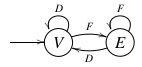
\includegraphics[scale=0.5]{img/skilift.png}

Zutaten: 

\begin{align*}
	A	&= (Q, \Sigma, \delta, q_0, F)  \\
	Q	&= \text{ Zustände} \\
	\Sigma	&= \text{ Alphabet} \\
	\delta	&= \text{ Übergangsfunktion (Pfeile)} \\
	q_0	&\in Q \text{, Startzustand (Initialisierung)} \\
	F	&\subset Q \text{, Akzeptierzustand}
\end{align*}

Zeichenbedeutungen:

$\delta$: Zustand, Zeichen $\rightarrow$ neuer Zustand.

$(q, a) \mapsto q'=\sigma(q,a)$

%$Q \multiply \Sigma \rightarrow^{\sigma} Q$

\subsection{Darstellung mittels Tabelle}

\begin{tabular}{c c}
 & $\Sigma$ \\
$Q$	& $\delta$
\end{tabular}

\subsection{Systematische Rekonstruierung aus der Sprache}

Zustände sind charakterisiert durch "was noch kommen darf"

\begin{align*}
	L(w) = \{v \in \Sigma^\ast | wv \in L \} \\
	\text{Beispiel: } \Sigma = \{a, b \}, L=\{ w \in \Sigma^\ast | |w|_a \text{ gerade}\}
\end{align*}


%TODO: Myhill-Nerode Tabelle mit Zuständen

\begin{align*}
W & L(w) \text{ (was kann angehängt werden)}\\
\varepsilon & L(\varepsilon) = \{v \in \Sigma^\ast | \varepsilon v \in L \} &= L \\
a & L(a) = \{v \in \Sigma^\ast | a v \in L \} &= \{ v \in \Sigma^\ast | |w|_a ungerade \}\\
b & L(b) = \{v \in \Sigma^\ast | b v \in L \} &= L\\
  & L(aa) &= L \\
  & L(ab) &= L(a) \\
  & L(ba) &= L(a) \\
  & L(bb) &= L
\end{align*}

\begin{enumerate}
	\item $L(w)$ ausrechnen: verschiedene $L(w)$ geben $Q$ 
	\item $\sigma: L(w) \rightarrow^a L(wa)$
	\item $q_0: L(\varepsilon) = L$
	\item $L(w)$ ist Akzeptierzustand wenn $\varepsilon \in L(w)$
\end{enumerate}

\subsection{Gleichheit von Automatensprachen feststellen}
	Reduktion auf Minimalautomat M$(A_1)$. Vereinfachung geht, indem zuerst die nicht-Equivalenten zuständige gemäss folgender Liste ausgeschlossen werden:

\begin{enumerate}
	\item Akzeptierzustand $\neq$ Nicht-Akzeptierzustand 
	\item Führt am $m$ Zustände $m$ ein nicht äquivalentes Paar über.
	\item Wiederholung des Algorithmus, bis keine Änderungen mehr auftreten.
	\item Restliche Zustände sind äquivalent.
\end{enumerate}

$\{0^n 1^n | n \geq 0\}$ nicht regulär (Myhill, qualvoll)

\subsubsection{Pumping Lemma}

Alle regulären Sprachen haben die Pumpeigenschaft (aber nicht zwingend umgekehrt).

$L$ regulär $\Rightarrow \exists N$ Punping Length, mit jedes Word $w \in L$ mit $|w| \geq N$ kann zerlegt werden $w=xyz$ mit 
\begin{enumerate}
	\item $|y| > 0$
	\item $|xy| \leq N$
	\item $xy^kz \in L, \forall k \in \mathbb{N}$
\end{enumerate}

\paragraph{Anwendung}

$L=\{0^n1^n|n \geq 0 \}$ ist nicht regulär. Widerspruchsbeweis:

\begin{enumerate}
	\item	Annahme: $L$ ist regulär
	\item	Pumping Lemma: $\exists N$
	\item	Konstruiere $W = 0^N1^N$, $|w| = 2N \geq N$, $w \in L$
	\item	Zerlegung: \\
			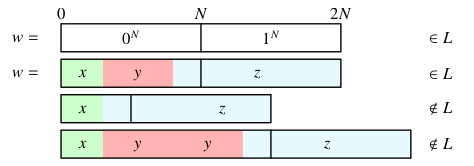
\includegraphics[scale=0.5]{img/pumpinglemma.png}
	\item	Pumpen: $k > 1 \Rightarrow xy^kz$ hat mehr $0$ als $1 \Rightarrow xy^kz \not\in L$ \Lightning $PL: xy^kz \in L$
	\item	Widerspruch: $L$ nicht regulär!
\end{enumerate}

\paragraph{Beispiel}
$\{w \in \varepsilon^\ast | w \text{ ist ein Palindrom }\}$ nicht regulär, $\varepsilon = \{0,1\}$

\begin{enumerate}
	\item	Annahme: $L$ regulär
	\item	PL: $\exists N$
	\item	Konstruiere ein Palindrom: $=0^N1^N1^N0^N$
	\item	Zerlegung: |/x/y/ 0 | 1  |  1 | 0 |
	\item	Pumpe: $k > 1, \Rightarrow xy^kz$ mehr $0$ links als rechts $\Rightarrow \not\in L$ \Lightning
	\item	Widerspruch: $L$ ist nicht regulär
\end{enumerate}

\subsection{Nicht deterministische Automaten}

\[
 \lambda : Q \times (\Sigma \cup \{\varepsilon\}) \rightarrow P(Q)
\]

$\cup \{\varepsilon\}$ ermöglich Sprünge; es können "Pfeile" weggelassen werden und es können mehrere Pfeile für den gleichen Buchstaben geben.

\paragraph{Beispiel} $L=\{ w \in \sigma^\ast | w \text{ beginnt und endet mit } 0\}$

%TODO: Graphik: ->kreis -0->kreis(selbstverweis für 0,1) -0-> doppelkreis

$w$ wird akzeptiert $\equiv \exists$  es gibt einen Weg, der auf einen Akzeptierzustand führt.

Aus so einem Graphen lässt sich immer einen endlichen Automaten konstruieren.


\subsection{$\text{NEA}_\varepsilon \to \text{DEA}$}

$\varepsilon$-Übergänge sind "gratis", d.h. verbrauchen kein Zeichen.


-> Alle Zustände / Kombinationen von Zuständen aufzeichnen
-> Alle Übergänge durchprobieren


\subsection{Mengenoperationen}
\subsubsection{Komplement}

Endzustände Streichen, alle anderen Zustände in Endzustände umwandeln.


\subsection{Reguläre Ausdrücke}

Ziel: Notation für reguläre Spraceh "reguläre Ausdrücke": $r$

\[
	L(r) = \{ w \in \Sigma^\ast | \text{ Wort } w \text{ passt auf den reg. Ausdruck } r\}
\]

Bausteine: primitiven reg. Ausrücke (Wörter mit höchstens 1 Zeichen)

\begin{tabular}{ l l}
	a & steht für $L(a) = \{ a \}$ \\
	. & steht für $L(.) = \{a,b,c\} = \{ w \ in \Sigma ^ \ast | |w| = 1 \}$\\
	$[0-9]$ & steht für $L([0-9])=\{w \in \{ 0, 1, ..., 9\}| |w| = 1 \}$\\
	$\varepsilon$ (leeres Wort) & steht für $L("") = \{ \varepsilon \}$
\end{tabular}

\subsubsection{Reguläre Operationen}

\begin{align*}
\text{Verkettung: } & L(r_1), L(r_2) \Rightarrow L(r_1,r_2) = L(r_1)L(r_2) \\
\text{Alternative: }& L(r_1),L(r_2) \Rightarrow L(r_1|r_2) = L(r_1) \cup L(r_2) \\
\text{*-Operation: }& L(r) \Rightarrow L(r^\ast) = L(r)^\ast
\end{align*}

\paragraph{Beispiel}

	\emph{(0 | (|-)[1-9][0-9]*)}  alternative Schreibweise \emph{-? r?} \\
	\emph{[0-9]+\.[0-9]+\.[0-9]+\.[0-9]}


\subsubsection{Umwandlung Automat / Ausdruck}
Umwandlung in einen Automat mit Startzustand $S$, einem Übergang $r$ und einen Akzepttierzustand $A$

Vorgehen, um einen Automaten in einen Ausdruck umzuwandeln:

\begin{itemize}
	\item Startzustand un Endzustand mittels $\varepsilon$-Übergängen hinzufügen.
	\item Zwischenzustände entfernen.
\end{itemize}

\section{Kontextfreie Grammatik}


Kann im Gegensatz zu Regulärer Sprache z.B. $\{0^n1^n | n \geq 0 \}$ darstellen. Dazu gehören alle moderne Programmiersprachen.

\paragraph{Beispiel Klammern $(()())$}

Mit Klammern können wir:

\begin{enumerate}
	\item $\varepsilon$ \hfill $A \to \varepsilon$
	\item Verketten \hfill $A \to AA$
	\item «Einklammern» \hfill $A \to (A)$
\end{enumerate}

diese 3 Regeln produzieren einen Klammerausdruck:
\[
	A \to (A) \to (AA) \to ((A)A) \to ((A)(A)) \to (()(A)) \to (()())
\]

\subsection{Definitionen}

\[
	G = (V, \Sigma, R, S)
\]

\begin{description}
	\item[$V$] \hfill \\
		Variable, Platzhalter für (Teil-)Ausdrücke
	\item[$\Sigma$] \hfill \\
		Terminalsymbole (Alphabet)
	\item[$R$] \hfill \\
		Regeln: $A \to BCx$ Zeichenkette von Variablen und Terminalsymbolen
	\item[$S$] \hfill \\
		Startvariable $S \in V$
\end{description}

Wir arbeiten \emph{Kontextfrei}, d.h. auf der linken Seite steht nur eine Variable.

Definition: $L$ kontextfrei $\Leftrightarrow L(G)  L$, $G$ kontextfreie Grammatik.


\paragraph{Beispiel I} \hfill \\
\[
	(\{A\}, \{(,)\}, \{A \to \varepsilon, A \to AA, A \to (A)\}, A)
\]

\paragraph{Beispiel: II}

Natürliche Zahlen ohne führende Nullen
\begin{align*}
	\text{Zahl} &\to \text{ziffer} \\
	\text{} &\to \text{ziffer} \\
	\text{ziffernfolge} &\to \text{ziffer} \\
	\text{} &\to \text{ziffernfolge ziffer}
\end{align*}

\begin{align*}
	\text{nichtnullziffer} &\to 1 | 2 | ... | 9 \\
	\text{ziffern} &\to 0 | \text{nichtnulziffer}
\end{align*}


\subsubsection{Notation}

$A \xRightarrow{\ast} w$

$w$ ensteht aus $A$ durch Regelanwendung. $w$ ist aus $A$ ableitbar.

\subsection{Voraussagbare Effizienz / Chomsky-Normalform}
Schlechte Ansätze:
\begin{itemize}
	\item Start auf der rechten Seite: Beliebig oft Schachteln.
	\item $\varepsilon$-Regeln: $A \to \varepsilon$ (Arbeit verrichten)
	\item Unit Rules: $A \to B$ (Endlosschleifen)
	\item $A \to u_1,u_2,...,u_n$ (Wortexplosionen)
\end{itemize}

Kochbuch guter Ansatz:

\begin{itemize}
	\item Startvariable nicht rechts
	\item $S \to \varepsilon$ als einzige $\varepsilon$-Regel
	\item Keine Unit Rules
	\item Nur Regeln der Form $A \to BC$ und $A \to a$
\end{itemize}

Forderung: $G$ heisst $m$ Chomsky-Normalform (CNF). In der CNF Braucht die Konstruktion von Wörtern $2 \cdot |w| -1$ Schritte.

 \subsection{Effizienter Parse-Algorithmus finden}
 
%TODO: Pseudo Algorythmus aus Script übernehmen

\subsection{Stackautomaten}

\begin{align*}
P &= (Q, \Sigma, \Gamma, \delta, q_0, F) \\
\Gamma & \\
\delta&: Q \times \Sigma_\varepsilon \times \Gamma_\varepsilon \to P(Q \times \Gamma) \\
\Sigma_\varepsilon &= \Sigma \cup \{ \varepsilon \}
\end{align*}

\subsubsection{Grammatik $\rightarrow$ Stackautomat}

\paragraph{Beispiel}

\[
L = \{ 0^n 1^n | n \geq 0 \}
\]

Grammatik:
\begin{align*}
S &\rightarrow 0S1 \\
  &\rightarrow \varepsilon
\end{align*}

Idee: Zwischenresultate der Produktionsregeln auf den Stack. Dies führt zur Konstruktion eines Stackautomaten, welcher immer vorzu matched, ob der Input der Sprache entspricht.



Am Anfang: $\varepsilon, \varepsilon \to \$; \varepsilon, \varepsilon \to S$


Von und zum Zentralen Punkt: 
\begin{align*}
A \to BC & \varepsilon, A \to c, \varepsilon, \varepsilon \to B \\
A \to a & \varepsilon, A \to a \\
S \to \varepsilon & \varepsilon, S \to \varepsilon \\
a, a \to \varepsilon & \text{(für jedes Terminalsymbol)} \\
\text{Am Ende:} & \varepsilon, \$ \to \varepsilon 
\end{align*}

\subsubsection{Stackautomat $\to$ Grammatik}

\begin{itemize}
	 \item Nur 1 Akzeptierzustand
	 \item Stack leer beim Akzeptieren (wegschmeissen von allem verbliebenem.
	 \item Bei jedem Übergang genau 1 Zeichen auf den Stack oder 1 Zeichen vom Stack (ersetzen von Zeichen nur über Umweg $\varepsilon$ möglich)
\end{itemize}

$w$ akzeptiert: es gibt einen Pfad durch den Stackautomaten von $q_0$ zu $q'_a$, Stack leer.

\begin{tabular}{l l l}
	Startvariable: & $S$&$=A_{q_0 q'_a}$ \\
	& $A_{pq}$&$= $ Wörter, die $p$ in $q$ überführen mit leerem Stack.
\end{tabular}

\paragraph{Spezialfälle}

Stack kommt irgendwann zwischendurch bei $r$ auf 0 $\Rightarrow A_{pq} \to A_{pr} A_{rq}$

Ein Wort vom Anfang des Stacks wird am Ende erst wieder abgebaut: $\Rightarrow A_{pq} \to a A_{rs} b$

\subsection{Backup-Naur-Form}

Standard für die Formulierung von Grammatiken.

Extended BNF: Wiederholungen, Kommentare etc.

\section{Turing-maschinen}

\end{document}